\documentclass[11pt,a4paper]{article}

\usepackage{amsmath,amssymb,amsthm}
\usepackage{mathtools}
\usepackage{bm}
\usepackage{enumerate}
\usepackage{hyperref}
\usepackage{cleveref}
\usepackage[margin=1in]{geometry}
\usepackage{tikz}
\usetikzlibrary{arrows.meta,calc,patterns,decorations.pathreplacing,fit}
\usepackage{pgfplots}
\pgfplotsset{compat=1.18}
\usepackage{tcolorbox}

% Theorem environments
\newtheorem{theorem}{Theorem}[section]
\newtheorem{lemma}[theorem]{Lemma}
\newtheorem{proposition}[theorem]{Proposition}
\theoremstyle{definition}
\newtheorem{definition}[theorem]{Definition}
\newtheorem{example}[theorem]{Example}
\newtheorem{remark}[theorem]{Remark}

% Notation shortcuts
\newcommand{\E}{\mathbb{E}}
\newcommand{\Var}{\mathrm{Var}}
\newcommand{\Normal}{\mathcal{N}}
\newcommand{\given}{\,|\,}
\newcommand{\btheta}{\boldsymbol{\theta}}
\newcommand{\bmu}{\boldsymbol{\mu}}
\DeclareMathOperator{\CE}{CE}

% Highlight box for key results
\newtcolorbox{keyresult}[1][]{
    colback=blue!5!white,
    colframe=blue!50!black,
    fonttitle=\bfseries,
    title={#1},
}

\title{The Jacobian Correction in Bayesian Inference:\\
A Detailed Guide}
\author{Technical Note}
\date{February 2026}

\begin{document}

\maketitle

\begin{abstract}
When a Bayesian prior is specified on a transformed quantity $Y = g(\theta)$
rather than the parameter $\theta$ directly, the induced prior on $\theta$
involves a Jacobian correction factor $|g'(\theta)|$. This note provides a
detailed, ground-up explanation of where this correction comes from, why it
has the form it does, and---crucially---why evaluating it requires only the
\emph{forward} mapping $g$ and its derivative, not the inverse $g^{-1}$. We
develop the 1D case with geometric intuition, extend to multiple dimensions,
show the complete Bayesian MCMC setup, and carefully analyze what goes wrong
when $g$ is not injective.
\end{abstract}

\tableofcontents
\newpage


%==============================================================================
\section{The Problem}
\label{sec:problem}
%==============================================================================

Consider the following situation. You have a model with parameter $\theta$
(or a parameter vector $\btheta$). The likelihood $p(\text{data} \given \theta)$
is naturally expressed in terms of $\theta$. But your prior beliefs are more
naturally expressed in terms of some transformed quantity $Y = g(\theta)$---for
instance, a certainty equivalent rather than a curvature parameter.

You specify a prior density $p_Y(y)$ on $Y$. Now you need $p_\theta(\theta)$,
the induced prior on $\theta$, so you can combine it with the likelihood to get
the posterior.

The standard answer involves a ``Jacobian correction'':
\begin{equation}
    \label{eq:main_formula}
    p_\theta(\theta) = p_Y\!\big(g(\theta)\big) \; \big|g'(\theta)\big|
\end{equation}
This note explains:
\begin{enumerate}
    \item Where this formula comes from (Sections~\ref{sec:discrete}--\ref{sec:1d}).
    \item Why it involves only the \emph{forward} map $g$ and its derivative, not
    the inverse $g^{-1}$ (Section~\ref{sec:forward_vs_inverse}).
    \item How it extends to multiple dimensions (Section~\ref{sec:multivariate}).
    \item How it fits into Bayesian MCMC (Section~\ref{sec:bayesian}).
    \item What goes wrong when $g$ is not injective
    (Section~\ref{sec:non_monotone}).
\end{enumerate}


%==============================================================================
\section{Warm-up: The Discrete Case}
\label{sec:discrete}
%==============================================================================

Before densities and Jacobians, consider the discrete case to build intuition.

Suppose $\theta \in \{1, 2, 3\}$ and $Y = g(\theta) = \theta^2$, so
$Y \in \{1, 4, 9\}$. If you specify a prior on $Y$:
\begin{equation}
    P(Y = 1) = 0.5, \quad P(Y = 4) = 0.3, \quad P(Y = 9) = 0.2
\end{equation}
then the induced prior on $\theta$ is immediate:
\begin{equation}
    P(\theta = 1) = P(Y = 1) = 0.5, \quad
    P(\theta = 2) = P(Y = 4) = 0.3, \quad
    P(\theta = 3) = P(Y = 9) = 0.2
\end{equation}
No correction is needed. Each value of $\theta$ maps to exactly one value of
$Y$, and the probability transfers directly:
$P(\theta = k) = P(Y = g(k))$.

The continuous case is different because probability is carried by
\emph{intervals}, not points, and intervals change size under nonlinear
transformations. That size change is what the Jacobian captures.


%==============================================================================
\section{The 1D Continuous Case}
\label{sec:1d}
%==============================================================================

\subsection{The Setup}

Let $Y = g(\theta)$ where $g$ is a smooth, strictly monotone function (we
handle the non-monotone case in Section~\ref{sec:non_monotone}). We have a
density $p_Y(y)$ on $Y$ and want the induced density $p_\theta(\theta)$ on
$\theta$.

\subsection{Derivation from First Principles}

The fundamental requirement is that probability is conserved: the probability
of $\theta$ falling in any interval must equal the probability of $Y$ falling
in the image of that interval. For a small interval $[\theta, \theta + d\theta]$:

\begin{equation}
    \label{eq:prob_conservation}
    \underbrace{p_\theta(\theta) \, d\theta}_{\text{prob in } \theta\text{-interval}}
    \;=\;
    \underbrace{p_Y(g(\theta)) \; |g'(\theta)| \, d\theta}_{\text{prob in the image } Y\text{-interval}}
\end{equation}

The right-hand side is the $Y$-density evaluated at $g(\theta)$, multiplied by
the \emph{length} of the image interval $|g'(\theta)| \, d\theta$. Canceling
$d\theta$ from both sides gives the formula:

\begin{keyresult}[The Jacobian Correction (1D)]
\begin{equation}
    \label{eq:1d_formula}
    p_\theta(\theta) = p_Y\!\big(g(\theta)\big) \; \big|g'(\theta)\big|
\end{equation}
\end{keyresult}

\subsection{Geometric Picture: Interval Stretching}

The Jacobian correction accounts for the fact that $g$ stretches or compresses
intervals. Figure~\ref{fig:stretching} illustrates this.

\begin{figure}[ht]
\centering
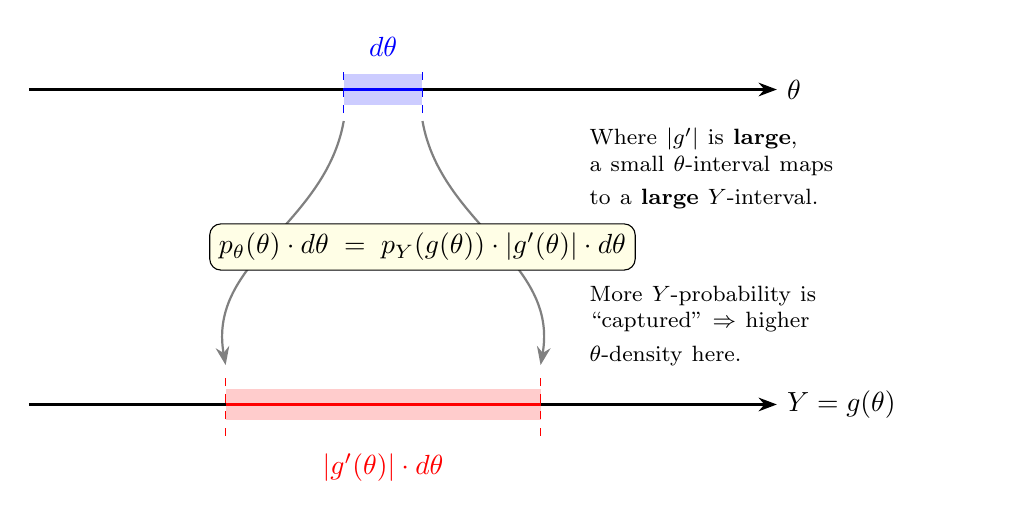
\begin{tikzpicture}[>=Stealth, scale=1.0]
    % theta axis (top)
    \draw[->, thick] (-0.5,4) -- (9,4) node[right] {$\theta$};
    % Y axis (bottom)
    \draw[->, thick] (-0.5,0) -- (9,0) node[right] {$Y = g(\theta)$};

    % Small interval on theta axis
    \fill[blue!20] (3.5,3.8) rectangle (4.5,4.2);
    \draw[very thick, blue] (3.5,4) -- (4.5,4);
    \draw[blue, dashed] (3.5,3.7) -- (3.5,4.3);
    \draw[blue, dashed] (4.5,3.7) -- (4.5,4.3);
    \node[blue, above] at (4,4.3) {$d\theta$};

    % Case 1: steep g (large |g'|) => wide image
    \fill[red!20] (2,-.2) rectangle (6,0.2);
    \draw[very thick, red] (2,0) -- (6,0);
    \draw[red, dashed] (2,-0.4) -- (2,0.4);
    \draw[red, dashed] (6,-0.4) -- (6,0.4);
    \node[red, below] at (4,-0.5) {$|g'(\theta)| \cdot d\theta$};

    % Arrows showing mapping
    \draw[->, thick, gray] (3.5,3.6) to[out=-100, in=100] (2,0.5);
    \draw[->, thick, gray] (4.5,3.6) to[out=-80, in=80] (6,0.5);

    % Labels
    \node[right, text width=5cm] at (6.5,3) {
        \footnotesize
        Where $|g'|$ is \textbf{large},\\
        a small $\theta$-interval maps\\
        to a \textbf{large} $Y$-interval.
    };
    \node[right, text width=5cm] at (6.5,1) {
        \footnotesize
        More $Y$-probability is\\
        ``captured'' $\Rightarrow$ higher\\
        $\theta$-density here.
    };

    % The key equation
    \node[draw, fill=yellow!10, rounded corners] at (4.5, 2) {
        $p_\theta(\theta) \cdot d\theta
        \;=\; p_Y(g(\theta)) \cdot |g'(\theta)| \cdot d\theta$
    };
\end{tikzpicture}
\caption{%
    A small interval of width $d\theta$ in parameter space maps to an interval
    of width $|g'(\theta)| \cdot d\theta$ in $Y$-space. The probability in the
    $Y$-interval (area under $p_Y$) equals the probability in the
    $\theta$-interval. When $|g'(\theta)|$ is large, the image interval is wide,
    capturing more probability from $p_Y$---so $p_\theta(\theta)$ must be
    correspondingly large.
}
\label{fig:stretching}
\end{figure}

The intuition: probability density is ``probability per unit length.'' When $g$
stretches a $\theta$-interval by a factor of $|g'(\theta)|$, the $Y$-interval
is $|g'(\theta)|$ times wider, so it contains $|g'(\theta)|$ times more
probability (approximately, for small intervals). That extra probability must
be accounted for in $p_\theta$.

\begin{example}[Linear transformation]
If $Y = a\theta + b$ with $a > 0$, then $g'(\theta) = a$ everywhere, and:
\begin{equation}
    p_\theta(\theta) = a \cdot p_Y(a\theta + b)
\end{equation}
A uniform prior on $Y \in [0, 10]$ induces a uniform prior on
$\theta \in [-b/a, (10-b)/a]$ with density $a \cdot (1/10) = a/10$. The
interval in $\theta$-space is $1/a$ times as wide, and the density is $a$
times as high---probability is conserved.
\end{example}

\begin{example}[Log transformation]
\label{ex:log}
If $Y = \log \theta$ (so $\theta > 0$), then $g'(\theta) = 1/\theta$. A
$\Normal(0, 1)$ prior on $Y$ induces:
\begin{equation}
    p_\theta(\theta) = \frac{1}{\theta} \cdot \frac{1}{\sqrt{2\pi}}
    e^{-(\log\theta)^2/2}
\end{equation}
which is the log-normal density. The $1/\theta$ factor makes the density
decay faster for large $\theta$---reflecting the fact that $\log$ compresses
large values (small $|g'|$) and stretches small values (large $|g'|$).
\end{example}


%==============================================================================
\section{Forward vs.\ Inverse: Two Forms of the Same Formula}
\label{sec:forward_vs_inverse}
%==============================================================================

This is where the confusion typically arises. The change-of-variables formula
can be written in two equivalent ways, and textbooks often present only one.

\subsection{The Two Directions}

Suppose $Y = g(\theta)$ is a smooth bijection. Then $\theta = g^{-1}(Y)$
exists.

\begin{keyresult}[Two equivalent forms]
\textbf{Forward form} (``I have $\theta$, I want $p_\theta(\theta)$''):
\begin{equation}
    \label{eq:forward}
    \boxed{p_\theta(\theta) = p_Y\!\big(g(\theta)\big) \; \big|g'(\theta)\big|}
\end{equation}

\vspace{6pt}
\textbf{Inverse form} (``I have $y$, I want $p_\theta$ at the corresponding
$\theta$''):
\begin{equation}
    \label{eq:inverse}
    p_\theta\!\big(g^{-1}(y)\big) = p_Y(y) \;
    \big|g'\!\big(g^{-1}(y)\big)\big|
    = \frac{p_Y(y)}{|(g^{-1})'(y)|}
\end{equation}
where the second equality uses the inverse function theorem:
$(g^{-1})'(y) = 1/g'(g^{-1}(y))$.

These are the \emph{same equation}---\eqref{eq:inverse} is just
\eqref{eq:forward} evaluated at $\theta = g^{-1}(y)$.
\end{keyresult}

The difference between the two forms is purely a matter of which variable you
start with.

\subsection{Which Do You Need?}

\begin{figure}[ht]
\centering
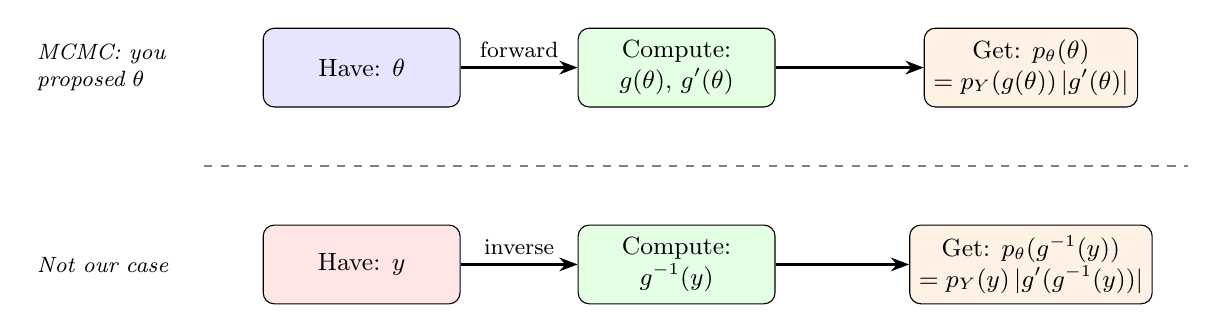
\begin{tikzpicture}[>=Stealth, scale=1.0,
    box/.style={draw, rounded corners, minimum height=1cm, minimum width=2.5cm,
    align=center, font=\small}]

    % Left scenario
    \node[box, fill=blue!10] (theta1) at (0, 2.5) {Have: $\theta$};
    \node[box, fill=green!10] (gtheta) at (4, 2.5) {Compute:\\$g(\theta)$, $g'(\theta)$};
    \node[box, fill=orange!10] (result1) at (8.5, 2.5) {Get: $p_\theta(\theta)$\\$= p_Y(g(\theta))\,|g'(\theta)|$};

    \draw[->, thick] (theta1) -- (gtheta) node[midway, above] {\footnotesize forward};
    \draw[->, thick] (gtheta) -- (result1);

    \node[left, text width=2.5cm, font=\footnotesize\itshape] at (-1.5, 2.5)
        {MCMC: you\\proposed $\theta$};

    % Right scenario
    \node[box, fill=red!10] (y1) at (0, 0) {Have: $y$};
    \node[box, fill=green!10] (ginv) at (4, 0) {Compute:\\$g^{-1}(y)$};
    \node[box, fill=orange!10] (result2) at (8.5, 0)
        {Get: $p_\theta(g^{-1}(y))$\\$= p_Y(y)\,|g'(g^{-1}(y))|$};

    \draw[->, thick] (y1) -- (ginv) node[midway, above] {\footnotesize inverse};
    \draw[->, thick] (ginv) -- (result2);

    \node[left, text width=2.5cm, font=\footnotesize\itshape] at (-1.5, 0)
        {Not our case};

    % Dividing line
    \draw[dashed, gray] (-2, 1.25) -- (10.5, 1.25);
\end{tikzpicture}
\caption{%
    \textbf{Top:} When you start with $\theta$ (the MCMC case), you only need
    the forward map $g$ and its derivative $g'$. \textbf{Bottom:} The inverse
    $g^{-1}$ is only needed if you start with $y$ and need to find the
    corresponding $\theta$.
}
\label{fig:forward_vs_inverse}
\end{figure}

The answer depends on what you start with:

\paragraph{Starting from $\theta$ (the MCMC case).} In Bayesian MCMC, your
sampler proposes a value of $\theta$. You need to evaluate $p_\theta(\theta)$.
Use the forward form \eqref{eq:forward}:
\begin{enumerate}
    \item Compute $g(\theta)$ --- the forward map.
    \item Evaluate $p_Y(g(\theta))$ --- plug the result into the known
        $Y$-density.
    \item Compute $|g'(\theta)|$ --- the derivative of the forward map.
    \item Multiply: $p_\theta(\theta) = p_Y(g(\theta)) \cdot |g'(\theta)|$.
\end{enumerate}
\textbf{No inverse is computed anywhere.}

\paragraph{Starting from $y$.} If instead someone hands you a value of $y$ and
asks ``what is $p_\theta$ at the corresponding $\theta$?'', then you need
$g^{-1}(y)$ to find out \emph{which} $\theta$ that is. This is when the
inverse appears. But in MCMC, you already have $\theta$---the sampler
proposed it.

\subsection{Why Textbooks Emphasize the Inverse}

Many probability textbooks present the change of variables in the ``other''
direction: given a density on $\theta$, find the density on $Y = g(\theta)$.
In that problem:
\begin{equation}
    p_Y(y) = p_\theta\!\big(g^{-1}(y)\big) \; \big|(g^{-1})'(y)\big|
\end{equation}
Here the inverse appears because you have $y$ but need to find the
corresponding $\theta$ to evaluate $p_\theta$. This is the textbook formula
that most people memorize, and it creates the impression that ``change of
variables always requires the inverse.''

For Bayesian prior specification, we are going the \emph{opposite} direction:
given a density on $Y$, induce a density on $\theta$. The inverse is not
needed.


%==============================================================================
\section{A Careful 1D Example}
\label{sec:example}
%==============================================================================

To make this fully concrete, consider the log transformation from
Example~\ref{ex:log}. Suppose we have a model parameter $\sigma > 0$ (a
standard deviation), and we specify our prior on $Y = \log \sigma$:
\begin{equation}
    Y \sim \Normal(0, 1)
\end{equation}
We want $p_\sigma(\sigma)$ so we can use it in MCMC where we sample $\sigma$
directly.

\paragraph{Step 1: The forward map.} $g(\sigma) = \log \sigma$, so
$g'(\sigma) = 1/\sigma$.

\paragraph{Step 2: Apply the formula.}
\begin{align}
    p_\sigma(\sigma) &= p_Y(g(\sigma)) \cdot |g'(\sigma)| \\
    &= p_Y(\log \sigma) \cdot \frac{1}{\sigma} \\
    &= \frac{1}{\sqrt{2\pi}} \exp\!\Big(-\frac{(\log \sigma)^2}{2}\Big)
    \cdot \frac{1}{\sigma}
\end{align}
This is the log-normal density. At no point did we need the inverse function
$g^{-1}(y) = e^y$.

\paragraph{Verification.} We can verify by computing the CDF:
\begin{align}
    P(\sigma \leq s) &= P(\log \sigma \leq \log s)
    = P(Y \leq \log s) = \Phi(\log s)
\end{align}
Differentiating: $p_\sigma(s) = \phi(\log s) / s$, where $\phi$ is the
standard normal density. This matches.

\paragraph{In MCMC.} Suppose the sampler proposes $\sigma = 2.5$. We compute:
\begin{align}
    g(2.5) &= \log 2.5 = 0.916 \\
    p_Y(0.916) &= \frac{1}{\sqrt{2\pi}} e^{-0.916^2/2} = 0.264 \\
    |g'(2.5)| &= 1/2.5 = 0.4 \\
    p_\sigma(2.5) &= 0.264 \times 0.4 = 0.106
\end{align}
All forward computations.

\begin{figure}[ht]
\centering
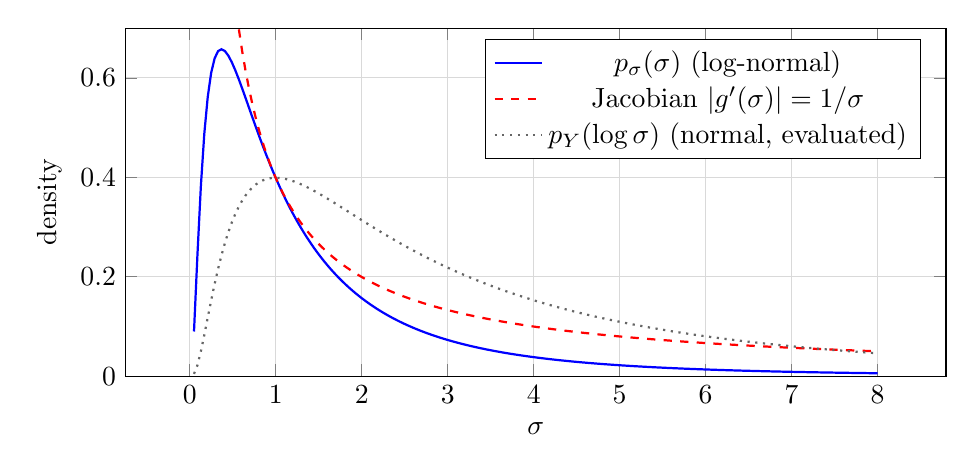
\begin{tikzpicture}
\begin{axis}[
    width=12cm, height=6cm,
    xlabel={$\sigma$}, ylabel={density},
    domain=0.05:8, samples=200,
    ymin=0, ymax=0.7,
    legend pos=north east,
    grid=major,
    grid style={gray!30},
]
\addplot[thick, blue] {1/(x*sqrt(2*pi)) * exp(-(ln(x))^2 / 2)};
\addlegendentry{$p_\sigma(\sigma)$ (log-normal)}

\addplot[thick, red, dashed] {1/(x*sqrt(2*pi))};
\addlegendentry{Jacobian $|g'(\sigma)| = 1/\sigma$}

\addplot[thick, black!60, dotted, domain=0.05:8]
    {1/sqrt(2*pi) * exp(-(ln(x))^2/2)};
\addlegendentry{$p_Y(\log\sigma)$ (normal, evaluated)}

\end{axis}
\end{tikzpicture}
\caption{%
    The log-normal density $p_\sigma(\sigma)$ (solid blue) is the product of
    the normal density $p_Y(\log\sigma)$ (dotted) and the Jacobian
    $1/\sigma$ (dashed red). For large $\sigma$, the Jacobian $1/\sigma$
    compresses the density; for small $\sigma$, it amplifies it. The normal
    density $p_Y(\log\sigma)$ alone (dotted) is \emph{not} a valid density on
    $\sigma > 0$---it doesn't integrate to 1 over $(0, \infty)$. The Jacobian
    correction makes it a proper density.
}
\label{fig:lognormal}
\end{figure}


%==============================================================================
\section{The Multivariate Case}
\label{sec:multivariate}
%==============================================================================

\subsection{From Derivatives to Determinants}

When $\btheta = (\theta_1, \ldots, \theta_p)$ and
$\mathbf{Y} = \mathbf{g}(\btheta) = (g_1(\btheta), \ldots, g_p(\btheta))$,
the scalar $|g'(\theta)|$ generalizes to the \emph{absolute determinant} of
the Jacobian matrix:
\begin{equation}
    J_{\mathbf{g}}(\btheta) =
    \begin{pmatrix}
        \partial g_1/\partial\theta_1 & \cdots & \partial g_1/\partial\theta_p \\
        \vdots & \ddots & \vdots \\
        \partial g_p/\partial\theta_1 & \cdots & \partial g_p/\partial\theta_p
    \end{pmatrix}
\end{equation}

\begin{keyresult}[The Jacobian Correction (Multivariate)]
\begin{equation}
    \label{eq:multi_formula}
    p_{\btheta}(\btheta) = p_{\mathbf{Y}}\!\big(\mathbf{g}(\btheta)\big) \;
    \big|\!\det J_{\mathbf{g}}(\btheta)\big|
\end{equation}
\end{keyresult}

The absolute determinant $|\!\det J_{\mathbf{g}}|$ is the multivariate analog
of $|g'|$: it measures how the mapping $\mathbf{g}$ scales \emph{volumes}
(rather than lengths) locally.

\subsection{Geometric Intuition: Volume Scaling}

In 1D, $|g'(\theta)|$ measures how $g$ stretches lengths. In $p$ dimensions,
$|\!\det J_{\mathbf{g}}(\btheta)|$ measures how $\mathbf{g}$ scales
$p$-dimensional volumes. Figure~\ref{fig:volume} illustrates the 2D case.

\begin{figure}[ht]
\centering
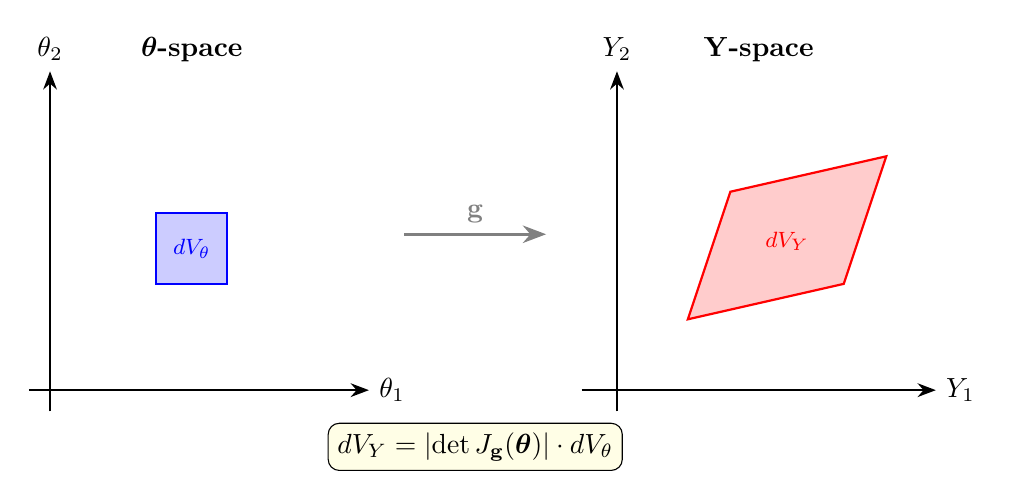
\begin{tikzpicture}[>=Stealth, scale=0.9]
    % Left: theta-space
    \node[above] at (2, 4.5) {\textbf{$\btheta$-space}};
    \draw[->, thick] (-0.3,0) -- (4.5,0) node[right] {$\theta_1$};
    \draw[->, thick] (0,-0.3) -- (0,4.5) node[above] {$\theta_2$};

    % Small square
    \fill[blue!20] (1.5,1.5) rectangle (2.5,2.5);
    \draw[thick, blue] (1.5,1.5) rectangle (2.5,2.5);
    \node[blue] at (2,2) {\footnotesize $dV_\theta$};

    % Arrow
    \draw[->, very thick, gray] (5, 2.2) -- (7, 2.2)
        node[midway, above] {$\mathbf{g}$};

    % Right: Y-space
    \begin{scope}[xshift=8cm]
    \node[above] at (2, 4.5) {\textbf{$\mathbf{Y}$-space}};
    \draw[->, thick] (-0.5,0) -- (4.5,0) node[right] {$Y_1$};
    \draw[->, thick] (0,-0.3) -- (0,4.5) node[above] {$Y_2$};

    % Parallelogram (image of the square under nonlinear map)
    \fill[red!20] (1,1) -- (3.2,1.5) -- (3.8,3.3) -- (1.6,2.8) -- cycle;
    \draw[thick, red] (1,1) -- (3.2,1.5) -- (3.8,3.3) -- (1.6,2.8) -- cycle;
    \node[red] at (2.4,2.1) {\footnotesize $dV_Y$};
    \end{scope}

    % Relationship
    \node[draw, fill=yellow!10, rounded corners] at (6, -0.8) {
        $dV_Y = |\!\det J_{\mathbf{g}}(\btheta)| \cdot dV_\theta$
    };
\end{tikzpicture}
\caption{%
    A small square in $\btheta$-space of volume $dV_\theta$ maps to a
    (generically) parallelogram in $\mathbf{Y}$-space of volume
    $|\!\det J_{\mathbf{g}}| \cdot dV_\theta$. The probability in the
    parallelogram under $p_{\mathbf{Y}}$ must equal the probability in the
    square under $p_{\btheta}$. This gives
    $p_{\btheta}(\btheta) = p_{\mathbf{Y}}(\mathbf{g}(\btheta)) \,
    |\!\det J_{\mathbf{g}}(\btheta)|$.
}
\label{fig:volume}
\end{figure}

The logic is identical to the 1D case:
\begin{itemize}
    \item A small box around $\btheta$ has volume $dV_\theta$.
    \item Its image under $\mathbf{g}$ has volume
        $|\!\det J_{\mathbf{g}}(\btheta)| \cdot dV_\theta$.
    \item The probability in that image is
        $p_{\mathbf{Y}}(\mathbf{g}(\btheta)) \cdot |\!\det J_{\mathbf{g}}| \cdot
        dV_\theta$.
    \item This must equal $p_{\btheta}(\btheta) \cdot dV_\theta$.
    \item Cancel $dV_\theta$:
        $p_{\btheta} = p_{\mathbf{Y}}(\mathbf{g}(\btheta)) \cdot
        |\!\det J_{\mathbf{g}}|$.
\end{itemize}

\subsection{What the Determinant Measures}

The columns of $J_{\mathbf{g}}$ are the images of the coordinate directions
under $\mathbf{g}$. The determinant measures the signed volume of the
parallelepiped they span:
\begin{itemize}
    \item $|\!\det J| > 1$: $\mathbf{g}$ \emph{expands} volumes locally.
    The $\btheta$-box maps to a larger $\mathbf{Y}$-region, capturing more
    $Y$-probability. So $p_{\btheta} > p_{\mathbf{Y}}(\mathbf{g}(\btheta))$.

    \item $|\!\det J| < 1$: $\mathbf{g}$ \emph{contracts} volumes. Less
    $Y$-probability is captured. So $p_{\btheta} < p_{\mathbf{Y}}(\mathbf{g}(\btheta))$.

    \item $|\!\det J| = 0$: $\mathbf{g}$ collapses the box to a lower
    dimension. The mapping is \emph{singular} at this point---see
    Section~\ref{sec:near_singular}.
\end{itemize}


%==============================================================================
\section{The Full Bayesian Setup}
\label{sec:bayesian}
%==============================================================================

Now we assemble everything for Bayesian posterior inference.

\subsection{The Ingredients}

\begin{enumerate}
    \item \textbf{Parameter:} $\btheta$ (e.g., risk preference parameters
    $r, \phi, \eta$).
    \item \textbf{Likelihood:} $p(\text{data} \given \btheta)$, expressed in
    terms of $\btheta$.
    \item \textbf{Prior on a transformation:} $p_{\mathbf{Y}}(\mathbf{y})$,
    where $\mathbf{Y} = \mathbf{g}(\btheta)$ (e.g., certainty equivalents).
    \item \textbf{Induced prior on $\btheta$:}
    $p_{\btheta}(\btheta) = p_{\mathbf{Y}}(\mathbf{g}(\btheta)) \,
    |\!\det J_{\mathbf{g}}(\btheta)|$.
\end{enumerate}

The posterior is:
\begin{equation}
    p(\btheta \given \text{data}) \propto
    \underbrace{p(\text{data} \given \btheta)}_{\text{likelihood}}
    \;\cdot\;
    \underbrace{p_{\mathbf{Y}}\!\big(\mathbf{g}(\btheta)\big)}_{\text{prior in }Y\text{-space}}
    \;\cdot\;
    \underbrace{\big|\!\det J_{\mathbf{g}}(\btheta)\big|}_{\text{Jacobian correction}}
\end{equation}

On the log scale (the natural form for MCMC):
\begin{equation}
    \label{eq:log_posterior}
    \log p(\btheta \given \text{data}) = \log p(\text{data} \given \btheta)
    + \log p_{\mathbf{Y}}\!\big(\mathbf{g}(\btheta)\big)
    + \log\big|\!\det J_{\mathbf{g}}(\btheta)\big| + \text{const.}
\end{equation}

\subsection{The MCMC Pipeline}

Figure~\ref{fig:pipeline} shows what happens at each MCMC step. The key
observation: every computation flows \emph{forward} from $\btheta$.

\begin{figure}[ht]
\centering
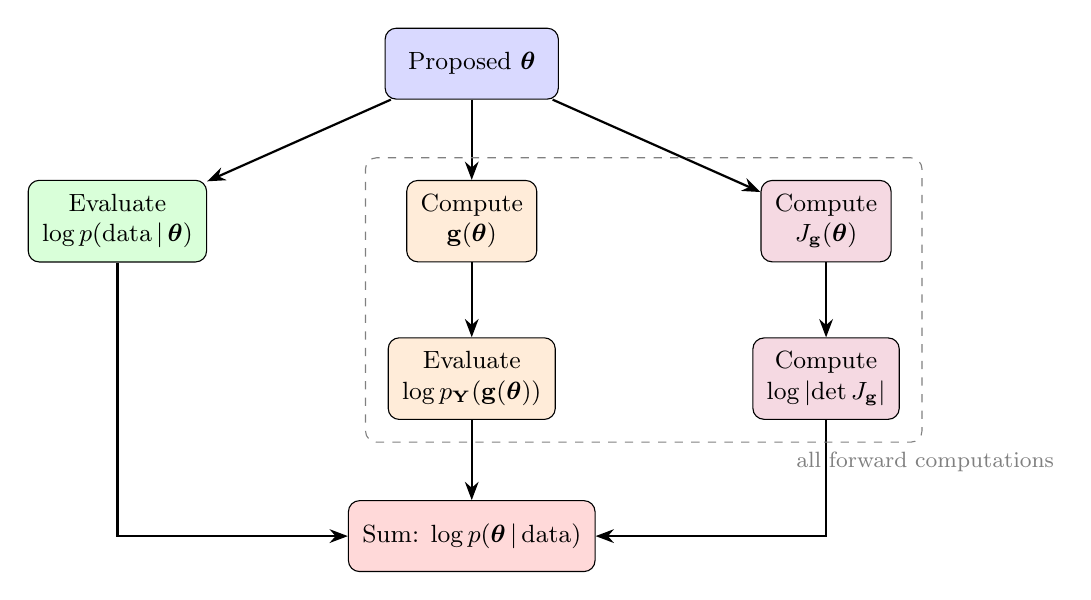
\begin{tikzpicture}[>=Stealth,
    box/.style={draw, rounded corners, minimum height=0.9cm,
    align=center, font=\small, inner sep=5pt},
    every node/.style={font=\small}]

    % Starting point
    \node[box, fill=blue!15, minimum width=2.2cm] (theta) at (0, 0)
        {Proposed $\btheta$};

    % Three branches
    % Branch 1: Likelihood
    \node[box, fill=green!15] (like) at (-4.5, -2)
        {Evaluate\\$\log p(\text{data} \given \btheta)$};

    % Branch 2: Forward map + prior
    \node[box, fill=orange!15] (geval) at (0, -2)
        {Compute\\$\mathbf{g}(\btheta)$};
    \node[box, fill=orange!15] (prior) at (0, -4)
        {Evaluate\\$\log p_{\mathbf{Y}}(\mathbf{g}(\btheta))$};

    % Branch 3: Jacobian
    \node[box, fill=purple!15] (jac) at (4.5, -2)
        {Compute\\$J_{\mathbf{g}}(\btheta)$};
    \node[box, fill=purple!15] (det) at (4.5, -4)
        {Compute\\$\log|\!\det J_{\mathbf{g}}|$};

    % Sum
    \node[box, fill=red!15, minimum width=3cm] (sum) at (0, -6)
        {Sum: $\log p(\btheta \given \text{data})$};

    % Arrows
    \draw[->, thick] (theta) -- (like);
    \draw[->, thick] (theta) -- (geval);
    \draw[->, thick] (theta) -- (jac);
    \draw[->, thick] (geval) -- (prior);
    \draw[->, thick] (jac) -- (det);
    \draw[->, thick] (like) |- (sum);
    \draw[->, thick] (prior) -- (sum);
    \draw[->, thick] (det) |- (sum);

    % Annotation
    \node[draw, dashed, gray, rounded corners, inner sep=8pt,
          fit=(geval)(prior)(jac)(det),
          label={[gray, font=\footnotesize]below right:all forward computations}] {};
\end{tikzpicture}
\caption{%
    The MCMC evaluation pipeline. Starting from a proposed $\btheta$, all
    computations flow forward: the likelihood is evaluated at $\btheta$, the
    forward map $\mathbf{g}(\btheta)$ feeds the $Y$-space prior, and the
    Jacobian is computed at $\btheta$. No inverse $\mathbf{g}^{-1}$ appears
    anywhere.
}
\label{fig:pipeline}
\end{figure}

\subsection{What Would Require the Inverse?}

The inverse $\mathbf{g}^{-1}$ is needed only if you sample in
$\mathbf{Y}$-space:
\begin{equation}
    \log p(\mathbf{Y} \given \text{data}) =
    \log p\!\big(\text{data} \given \mathbf{g}^{-1}(\mathbf{Y})\big)
    + \log p_{\mathbf{Y}}(\mathbf{Y})
    + \text{const.}
\end{equation}
Here the likelihood needs $\btheta = \mathbf{g}^{-1}(\mathbf{Y})$, which
requires solving a nonlinear system at each step. The prior is trivial (just
$p_{\mathbf{Y}}$, no Jacobian) but the likelihood evaluation requires inversion.

By sampling in $\btheta$-space instead, the likelihood is trivial and the
prior requires a Jacobian but no inversion. Since the Jacobian is a closed-form
expression (or computed cheaply via autodiff), this is strictly preferable.

\subsection{Automatic Differentiation}

In practice, you do not need to derive the Jacobian by hand. Given a function
\texttt{g(theta)} implemented in a differentiable framework (JAX, PyTorch),
automatic differentiation computes the exact Jacobian matrix:
\begin{verbatim}
    J = jax.jacfwd(g)(theta)       # 3x3 Jacobian matrix
    log_det = jnp.log(jnp.abs(jnp.linalg.det(J)))
\end{verbatim}
This is exact (not a finite-difference approximation) and has computational
cost roughly proportional to $p$ forward evaluations of $\mathbf{g}$.

For the RDU application with $p = 3$ preference parameters and 3 reference
lotteries, the Jacobian is a $3 \times 3$ matrix. Computing its determinant is
negligible relative to the likelihood evaluation over 80 choice observations.


%==============================================================================
\section{The Hierarchical (BHM) Extension}
\label{sec:bhm}
%==============================================================================

In the hierarchical model of the companion paper, each subject $i$ has their
own parameters $\btheta_i$, with a population-level prior. The Jacobian
correction applies \emph{per subject}.

\subsection{Setup}

The prior hierarchy in $\mathbf{Y}$-space is:
\begin{align}
    Y_i^k \given \mu_k^Y, \sigma_k^{Y2} &\sim \Normal(\mu_k^Y, \sigma_k^{Y2})
    \\
    \mu_k^Y &\sim \Normal(\mu_{0,k}^Y, \tau_{0,k}^{Y2}) \\
    \sigma_k^{Y2} &\sim \text{IG}(\alpha_0, \beta_{0,k}^Y)
\end{align}
where $\mathbf{Y}_i = \mathbf{g}(\btheta_i)$ are certainty equivalents. The
hyperparameters $(\mu_k^Y, \sigma_k^{Y2})$ live in $\mathbf{Y}$-space and
require no Jacobian correction---they are not transformed.

\subsection{The Log-Posterior}

For subject $i$, sampling $\btheta_i$ in parameter space:
\begin{equation}
    \label{eq:bhm_log_posterior}
    \log p(\btheta_i \given \mu^Y, \sigma^{Y2}, \text{data}_i) =
    \log p(\text{data}_i \given \btheta_i)
    + \sum_{k=1}^p \log \phi\!\left(\frac{g_k(\btheta_i) - \mu_k^Y}
    {\sigma_k^Y}\right) - \log \sigma_k^Y
    + \log\big|\!\det J_{\mathbf{g}}(\btheta_i)\big| + \text{const.}
\end{equation}
where $\phi$ is the standard normal density. The three terms are:
\begin{enumerate}
    \item The likelihood---how well $\btheta_i$ explains subject $i$'s choices.
    \item The hierarchical prior---how consistent $\btheta_i$'s implied CEs are
    with the population distribution.
    \item The Jacobian---the correction for working in $\btheta$-space rather
    than $\mathbf{Y}$-space.
\end{enumerate}

The hyperparameters $(\mu_k^Y, \sigma_k^{Y2})$ are sampled with their own
priors (normal and inverse-gamma), with no Jacobian involved---they are
sampled in the same space where their priors are specified.


%==============================================================================
\section{When $g$ Is Not Monotone (Not Injective)}
\label{sec:non_monotone}
%==============================================================================

Everything above assumed $\mathbf{g}$ is a diffeomorphism---a smooth bijection
with smooth inverse. What happens when this fails?

\subsection{The 1D Problem: \texorpdfstring{$g(\theta) = \theta^2$}{g(theta) = theta squared}}

Consider $\theta \in \mathbb{R}$ and $Y = g(\theta) = \theta^2$. This is not
injective: both $\theta = 2$ and $\theta = -2$ map to $Y = 4$.

\begin{figure}[ht]
\centering
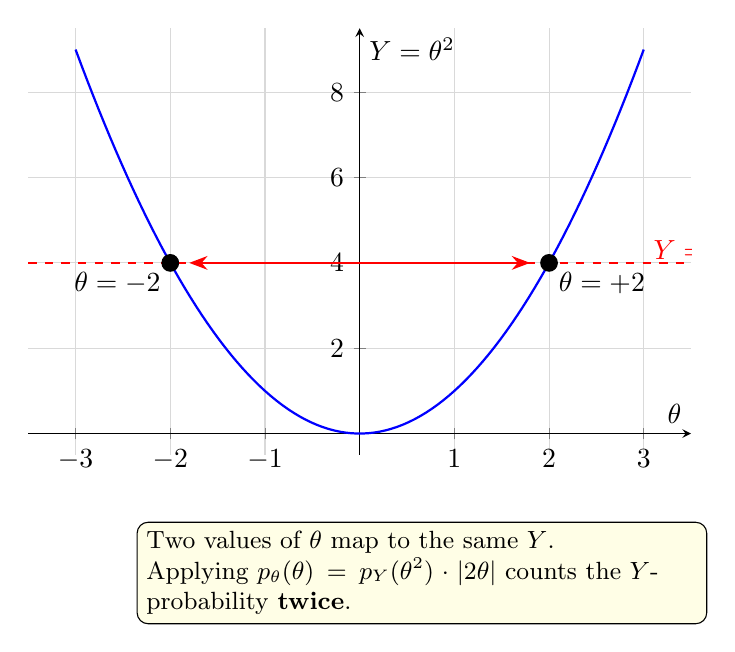
\begin{tikzpicture}[>=Stealth]
\begin{axis}[
    width=10cm, height=7cm,
    xlabel={$\theta$}, ylabel={$Y = \theta^2$},
    domain=-3:3, samples=100,
    ymin=-0.5, ymax=9.5,
    xmin=-3.5, xmax=3.5,
    grid=major,
    grid style={gray!30},
    axis lines=middle,
]
    % The parabola
    \addplot[thick, blue] {x^2};

    % Horizontal line at y=4
    \addplot[thick, red, dashed] coordinates {(-3.5,4) (3.5,4)};
    \node[red, right] at (axis cs:3.0,4.3) {$Y = 4$};

    % Mark the two preimages
    \addplot[only marks, mark=*, mark size=3pt, black]
        coordinates {(-2,4) (2,4)};
    \node[below left] at (axis cs:-2,4) {$\theta = -2$};
    \node[below right] at (axis cs:2,4) {$\theta = +2$};

    % Arrows pointing to both preimages
    \draw[->, thick, red] (axis cs:0,4) -- (axis cs:-1.8,4);
    \draw[->, thick, red] (axis cs:0,4) -- (axis cs:1.8,4);

\end{axis}

\node[draw, rounded corners, fill=yellow!10, text width=7cm, align=left,
      font=\small] at (5, -1.5) {
    Two values of $\theta$ map to the same $Y$.\\
    Applying $p_\theta(\theta) = p_Y(\theta^2) \cdot |2\theta|$
    counts the $Y$-probability \textbf{twice}.
};
\end{tikzpicture}
\caption{%
    The mapping $g(\theta) = \theta^2$ is not injective: every $Y > 0$ has
    two preimages $\pm\sqrt{Y}$. Naively applying the Jacobian formula
    $p_\theta(\theta) = p_Y(\theta^2) \cdot |2\theta|$ produces a function
    that integrates to 2, not 1---each $Y$-value's probability is counted once
    for each preimage.
}
\label{fig:non_injective}
\end{figure}

If we naively apply the formula $p_\theta(\theta) = p_Y(\theta^2) \cdot
|2\theta|$, we get a function that integrates to:
\begin{equation}
    \int_{-\infty}^{\infty} p_Y(\theta^2) \, |2\theta| \, d\theta
    = 2 \int_0^{\infty} p_Y(y) \, dy = 2
\end{equation}
(using the substitution $y = \theta^2$). The probability is doubled because
every $Y$-value has two preimages, each contributing the full
$Y$-probability.

\subsection{Why the Forward Pass Is Insufficient}

This is the critical point. The forward pass at a proposed $\theta$ gives you
two things: $g(\theta)$ and $|g'(\theta)|$. From these you compute
$p_Y(g(\theta)) \cdot |g'(\theta)|$. But this computation tells you
\textbf{nothing} about whether other values $\theta' \neq \theta$ also satisfy
$g(\theta') = g(\theta)$. The forward evaluation is entirely local---it has no
way to detect that $\theta = -2$ and $\theta = +2$ both produce $Y = 4$.

This is precisely why the formula breaks. The derivation in
Section~\ref{sec:1d} assumes that probability in a small $\theta$-interval
equals probability in its image $Y$-interval. When $g$ is injective, each
$Y$-interval is the image of exactly one $\theta$-interval, so the accounting
is correct. When $g$ is not injective, multiple $\theta$-intervals map to
\emph{overlapping} $Y$-intervals. The formula assigns the full
$Y$-probability to each preimage, but that probability is shared among them---it
should be split, not duplicated.

Detecting and correcting for non-injectivity requires \emph{global} information
about $g$: either explicit knowledge of the inverse (to enumerate all
preimages), or a proof that only one preimage exists on the relevant domain.
The Jacobian being nonzero at $\theta$ guarantees only \emph{local}
injectivity---no \emph{nearby} $\theta'$ maps to the same $Y$---but says
nothing about distant $\theta'$ values. Section~\ref{sec:verifying} discusses
how to establish global injectivity.

\subsection{The Correct Formula for Non-Injective \texorpdfstring{$g$}{g}}

When going from a $\theta$-density to a $Y$-density with a non-injective $g$,
the correct formula sums over preimages:
\begin{equation}
    \label{eq:sum_preimages}
    p_Y(y) = \sum_{k} \frac{p_\theta(\theta_k)}{|g'(\theta_k)|}
    \qquad \text{where } \{\ \theta_k : g(\theta_k) = y\ \}
\end{equation}
But going the other direction---from $p_Y$ to $p_\theta$---is
\textbf{not well-defined} without additional information. The problem is
fundamental: a density on $Y$ does not uniquely determine a density on
$\theta$ when $g$ is non-injective. How should the probability of $Y = 4$ be
split between $\theta = -2$ and $\theta = +2$? The answer depends on
information not contained in $p_Y$ alone.

\subsection{Resolution: Restrict to an Injective Region}

In practice, the solution is straightforward: ensure that $\mathbf{g}$ is
injective on the support of the prior. For the RDU application, this means:

\begin{enumerate}
    \item The parameter space is already restricted: $r > 0$, $\phi > 0$,
    $\eta > 0$.
    \item The CE mapping $\mathbf{g}(r, \phi, \eta) = (\CE_1, \CE_2, \CE_3)$
    should be verified to be injective on this restricted domain.
    \item As shown in the companion note, this holds when the reference
    lotteries have distinct cumulative probability structures.
\end{enumerate}

When $\mathbf{g}$ is injective on the relevant domain, the Jacobian formula
\eqref{eq:multi_formula} is valid and produces a properly normalized density.


%==============================================================================
\section{Near-Singular Jacobian}
\label{sec:near_singular}
%==============================================================================

Even when $\mathbf{g}$ is technically injective, problems arise if
$|\!\det J_{\mathbf{g}}|$ is very small or zero at some points.

\subsection{What \texorpdfstring{$\det J = 0$}{det J = 0} Means Geometrically}

When $\det J_{\mathbf{g}}(\btheta) = 0$ at a point, the mapping $\mathbf{g}$
locally collapses a $p$-dimensional region to something lower-dimensional. In
1D: $g'(\theta_0) = 0$ means $g$ has a local extremum at $\theta_0$---the
mapping ``folds'' at that point.

\begin{figure}[ht]
\centering
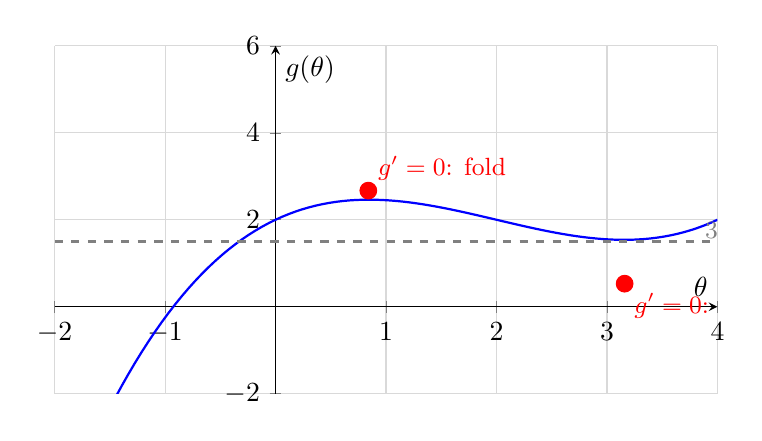
\begin{tikzpicture}[>=Stealth]
\begin{axis}[
    width=10cm, height=6cm,
    xlabel={$\theta$}, ylabel={$g(\theta)$},
    domain=-2:4, samples=100,
    ymin=-2, ymax=6,
    grid=major,
    grid style={gray!30},
    axis lines=middle,
]
    % A non-monotone function with a local max and min
    \addplot[thick, blue] {0.15*x^3 - 0.9*x^2 + 1.2*x + 2};

    % Mark the critical points (where g'=0)
    % g'(x) = 0.45x^2 - 1.8x + 1.2 = 0 => x = (1.8 +/- sqrt(3.24-2.16))/0.9
    % = (1.8 +/- 1.04)/0.9 => x = 0.84 or x = 3.16
    \addplot[only marks, mark=*, mark size=3pt, red]
        coordinates {(0.84, 2.67) (3.16, 0.53)};

    \node[red, above right, font=\small] at (axis cs:0.84, 2.67)
        {$g'= 0$: fold};
    \node[red, below right, font=\small] at (axis cs:3.16, 0.53)
        {$g'= 0$: fold};

    % Horizontal line showing three preimages
    \addplot[thick, dashed, gray] coordinates {(-2,1.5) (4,1.5)};
    \node[gray, right, font=\small] at (axis cs:3.8,1.7) {3 preimages};

\end{axis}
\end{tikzpicture}
\caption{%
    A non-monotone function with two critical points (folds). At these points,
    $g'(\theta) = 0$ and the Jacobian formula gives
    $p_\theta(\theta) = p_Y(g(\theta)) \cdot 0 = 0$---the induced prior
    density vanishes. Between the folds, some $Y$-values have 3 preimages,
    and the naive formula overcounts.
}
\label{fig:folds}
\end{figure}

\subsection{Implications for MCMC}

If $\det J_{\mathbf{g}} = 0$ at a point in the parameter space:
\begin{itemize}
    \item The induced prior density is zero there:
    $p_{\btheta}(\btheta) = p_{\mathbf{Y}}(\mathbf{g}(\btheta)) \cdot 0 = 0$.
    \item The log-prior is $-\infty$, so the MCMC sampler will reject
    proposals near that point.
    \item This is usually correct behavior: a fold in $\mathbf{g}$ means
    that nearby parameter values produce nearly identical observables, so they
    are effectively unidentifiable.
\end{itemize}

If $\det J_{\mathbf{g}}$ is very small but nonzero, the induced prior strongly
penalizes that region. This is also usually appropriate: it reflects the fact
that the mapping ``compresses'' the parameter space there, making it hard to
distinguish nearby parameter values from their observable consequences.

\subsection{When the Jacobian Changes Sign}

If $\det J_{\mathbf{g}}$ changes sign across the parameter space, it means the
mapping reverses orientation somewhere---a topological obstruction to global
injectivity. The absolute value $|\!\det J|$ is continuous and nonneg\-ative, so
it passes through zero at sign changes. These zeros are exactly the folds
where injectivity breaks down.

For the RDU-Prelec CE mapping, the companion note verified that
$\det J > 0$ at all tested points in the relevant parameter region, providing
numerical evidence that no such folds exist.


%==============================================================================
\section{Verifying Injectivity}
\label{sec:verifying}
%==============================================================================

The Jacobian formula requires $\mathbf{g}$ to be injective on the prior
support. This section surveys the available tools for establishing injectivity,
from elementary results to general theorems applicable to complex nonlinear
mappings.

\subsection{Local vs.\ Global Injectivity}

The inverse function theorem guarantees that if
$\det J_{\mathbf{g}}(\btheta_0) \neq 0$ at a point $\btheta_0$, then
$\mathbf{g}$ is injective on some \emph{neighborhood} of $\btheta_0$. This is
\textbf{local} injectivity---it says no nearby $\btheta'$ produces the same
$\mathbf{Y}$, but says nothing about distant $\btheta'$.

\textbf{Global} injectivity---$\mathbf{g}(\btheta) = \mathbf{g}(\btheta')$
implies $\btheta = \btheta'$ for \emph{all} $\btheta, \btheta'$ in the
domain---is a strictly stronger property. The gap between local and global
is exactly the $\theta^2$ problem: $g'(\theta) \neq 0$ everywhere except
$\theta = 0$, so $g$ is locally injective almost everywhere, but globally it
is not.

The relationship between $\det J$ and global injectivity is:
\begin{center}
\begin{tabular}{lcc}
    Condition & Local injectivity & Global injectivity \\
    \hline
    $\det J \neq 0$ at a point & at that point & no \\
    $\det J \neq 0$ everywhere & everywhere & \textbf{not necessarily} \\
    $\det J \neq 0$ everywhere + additional condition & everywhere & \textbf{yes} \\
\end{tabular}
\end{center}
The ``additional condition'' is the subject of the rest of this section.


\subsection{One Dimension: Monotonicity}

In 1D, global injectivity is equivalent to \emph{strict monotonicity}, which is
equivalent to $g'$ maintaining a constant sign:
\begin{equation}
    g \text{ injective on } I \quad\Longleftrightarrow\quad
    g'(\theta) > 0 \;\forall\, \theta \in I
    \quad\text{or}\quad g'(\theta) < 0 \;\forall\, \theta \in I
\end{equation}
(for continuously differentiable $g$ on an interval $I$). This is the simplest
and most commonly used test. Note that $g'(\theta) \neq 0$ everywhere is
necessary but not sufficient---it guarantees no local extrema, but on a
disconnected domain, $g$ could still fail to be injective.


\subsection{Hadamard's Global Inverse Function Theorem}

The most powerful general result is Hadamard's theorem, which adds one
topological condition to the local inverse function theorem:

\begin{theorem}[Hadamard, 1906]
\label{thm:hadamard}
Let $\mathbf{g}: \mathbb{R}^p \to \mathbb{R}^p$ be a $C^1$ mapping. If:
\begin{enumerate}
    \item $\det J_{\mathbf{g}}(\btheta) \neq 0$ for all $\btheta \in
    \mathbb{R}^p$ \emph{(local diffeomorphism)}, and
    \item $\|\mathbf{g}(\btheta)\| \to \infty$ as
    $\|\btheta\| \to \infty$ \emph{(properness/coercivity)},
\end{enumerate}
then $\mathbf{g}$ is a global diffeomorphism: it is bijective, and its inverse
$\mathbf{g}^{-1}$ is also $C^1$.
\end{theorem}

The properness condition says that $\mathbf{g}$ ``sends infinity to
infinity''---it cannot map a sequence escaping to infinity back to a bounded
region. This rules out pathological cases like $g(\theta) = \theta +
\sin(\theta)$ (which is a local but not global diffeomorphism in 1D---actually
this one is, but $g(\theta) = e^{i\theta}$ on the real line maps to the
unit circle, compressing infinity to a bounded set).

For economic applications, properness is often easy to verify:
\begin{itemize}
    \item If each component $g_k$ is dominated by a term that grows without
    bound as any parameter goes to its boundary, properness holds.
    \item For CE mappings: as $r \to \infty$, the CE approaches the minimum
    prize; as $r \to -\infty$, it approaches the maximum prize. The CEs are
    bounded, so technically Hadamard's theorem doesn't apply directly. However,
    one can apply it on a bounded domain (see the remark below).
\end{itemize}

\begin{remark}[Bounded domains]
Hadamard's theorem extends to open bounded domains $\Omega$: if $\mathbf{g}$ is
a local diffeomorphism on $\Omega$ and is \emph{proper relative to $\Omega$}
(meaning $\mathbf{g}^{-1}(K) \cap \Omega$ is compact for every compact
$K \subset \mathbf{g}(\Omega)$), then $\mathbf{g}$ is injective on $\Omega$.
In practice, this means $\mathbf{g}$ doesn't map interior sequences to boundary
points of the image.
\end{remark}


\subsection{The Gale--Nikaido Theorem}

For mappings on convex domains, there is a purely algebraic sufficient
condition:

\begin{theorem}[Gale--Nikaido, 1965]
\label{thm:gale_nikaido}
Let $\Omega \subset \mathbb{R}^p$ be open and \textbf{convex}. If the Jacobian
$J_{\mathbf{g}}(\btheta)$ is a \textbf{P-matrix} for all $\btheta \in \Omega$
(i.e., all principal minors of $J_{\mathbf{g}}$ are positive), then
$\mathbf{g}$ is injective on $\Omega$.
\end{theorem}

The P-matrix condition is stronger than $\det J > 0$. For a $3 \times 3$
Jacobian, it requires:
\begin{enumerate}
    \item All diagonal entries positive:
    $\partial g_k / \partial \theta_k > 0$ for $k = 1, 2, 3$.
    \item All $2 \times 2$ principal minors positive (there are 3 of these).
    \item The full determinant positive: $\det J > 0$.
\end{enumerate}
This is checkable analytically or numerically. The convexity of $\Omega$ is
essential---on non-convex domains, the theorem fails.

For economic mappings, the P-matrix condition has a natural interpretation:
each output $g_k$ responds positively to its ``own'' input $\theta_k$ (the
diagonal entries), and the cross-effects are not too large (the minor
conditions). This is related to the gross substitutes condition in demand
theory.

\begin{remark}[Weaker variant]
If $J_{\mathbf{g}}(\btheta) + J_{\mathbf{g}}(\btheta)^\top$ is positive
definite for all $\btheta \in \Omega$ (i.e., the symmetric part of the
Jacobian is PD), then $\mathbf{g}$ is \emph{strongly monotone} and hence
injective on any (not necessarily convex) domain. This is often easier to
check but is a stronger requirement than the P-matrix condition.
\end{remark}


\subsection{Constant-Sign Determinant on Simply Connected Domains}

A middle ground between the local inverse function theorem and the full
Gale--Nikaido/Hadamard results:

\begin{proposition}
\label{prop:constant_sign}
Let $\Omega \subset \mathbb{R}^p$ be open, bounded, and simply connected
(no holes). If $\det J_{\mathbf{g}}(\btheta) \neq 0$ for all
$\btheta \in \overline{\Omega}$ (the closure), and $\mathbf{g}$ is injective
on $\partial\Omega$ (the boundary), then $\mathbf{g}$ is injective on $\Omega$.
\end{proposition}

This follows from topological degree theory: the degree of $\mathbf{g}$ is
constant on connected components of $\mathbb{R}^p \setminus
\mathbf{g}(\partial\Omega)$, and if the boundary is mapped injectively, the
degree is $\pm 1$, which combined with local injectivity gives global
injectivity.

In practice, this means: if you can verify $\det J \neq 0$ on a compact
domain and check injectivity on the boundary (a lower-dimensional problem),
you get global injectivity on the interior.


\subsection{Structural Analysis: Exploiting Function Composition}

For complex mappings, it is often productive to decompose $\mathbf{g}$ into
simpler pieces and verify injectivity of each:

\paragraph{Composition.} If $\mathbf{g} = \mathbf{h} \circ \mathbf{f}$ and
both $\mathbf{h}$ and $\mathbf{f}$ are injective, then $\mathbf{g}$ is
injective. This is useful when $\mathbf{g}$ has a natural layered structure.

\paragraph{Triangular maps.} If $\mathbf{g}$ has a triangular structure:
\begin{align}
    g_1 &= g_1(\theta_1) \\
    g_2 &= g_2(\theta_1, \theta_2) \\
    g_3 &= g_3(\theta_1, \theta_2, \theta_3)
\end{align}
then injectivity of $\mathbf{g}$ reduces to: $g_1$ is injective in $\theta_1$,
$g_2$ is injective in $\theta_2$ for each fixed $\theta_1$, and $g_3$ is
injective in $\theta_3$ for each fixed $(\theta_1, \theta_2)$. The Jacobian of
a triangular map is triangular, so $\det J$ is the product of diagonal entries,
and the P-matrix condition reduces to checking each diagonal entry is positive.

\paragraph{Separable components.} If $g_k$ depends only on $\theta_k$ (the
fully diagonal case), then injectivity of $\mathbf{g}$ is equivalent to
injectivity of each $g_k$ individually---the 1D monotonicity test applied
component by component.

\paragraph{Monotone transformations of outputs.} If
$\mathbf{h}(\mathbf{Y}) = (h_1(Y_1), \ldots, h_p(Y_p))$ with each $h_k$
strictly monotone, then $\mathbf{h} \circ \mathbf{g}$ is injective if and only
if $\mathbf{g}$ is. This is why the RDU analysis works with
$B_k = (1-r) \cdot \text{RDU}_k$ instead of $\CE_k$---the monotone
transformation $\CE_k = B_k^{1/(1-r)}$ preserves injectivity.


\subsection{Red Flags Suggesting Non-Injectivity}

Before attempting a formal proof, look for structural warning signs:

\begin{enumerate}
    \item \textbf{Symmetric parameter entry.} If $g(\theta_1, \theta_2) =
    g(\theta_2, \theta_1)$---i.e., two parameters enter symmetrically---then
    $\mathbf{g}$ maps $(\theta_1, \theta_2)$ and $(\theta_2, \theta_1)$ to the
    same point. The $\theta^2$ example is the 1D version: $g(\theta) = g(-\theta)$.

    \item \textbf{Lower-dimensional intermediates.} If two parameters enter
    only through a single intermediate quantity---e.g., $\phi$ and $\eta$ enter
    only through $\phi \cdot \eta$---then varying $\phi$ and $\eta$ while holding
    $\phi\eta$ fixed produces the same output. This is why the Prelec PWF
    $w(p) = \exp(-\eta(-\ln p)^\phi)$ is important: $\phi$ and $\eta$ enter
    through \emph{different} functional forms, not a single product.

    \item \textbf{Bounded outputs from unbounded inputs.} If all components of
    $\mathbf{g}$ are bounded (as CEs are, by the prize range), then
    $\mathbf{g}$ maps $\mathbb{R}^p$ into a bounded region, which is
    impossible for a bijection $\mathbb{R}^p \to \mathbb{R}^p$. This means
    injectivity can only hold on a restricted domain, not globally on all of
    $\mathbb{R}^p$. This is usually fine for economic parameters, which have
    natural bounds.

    \item \textbf{Periodic components.} If any component of $\mathbf{g}$ is
    periodic in any parameter---e.g., $g_1 = \sin(\theta_1)$---then
    $\mathbf{g}$ cannot be globally injective.

    \item \textbf{Critical points of components.} If $\partial g_k / \partial
    \theta_j = 0$ at some interior point for all $j$, then $g_k$ has a critical
    point. The Jacobian has a zero row there, so $\det J = 0$ and local
    injectivity fails.
\end{enumerate}


\subsection{Practical Verification Strategies}

For a specific mapping $\mathbf{g}$, the following escalating sequence of
checks is recommended:

\paragraph{Step 1: Structural analysis.} Check for the red flags above. If the
mapping has symmetric parameter entry or lower-dimensional intermediates, stop:
it is not injective without domain restriction.

\paragraph{Step 2: Compute the Jacobian symbolically.} If possible, derive
$J_{\mathbf{g}}$ in closed form (or have a CAS like SymPy do it). Inspect
the diagonal entries $\partial g_k / \partial \theta_k$---these should have
a definite sign on the domain of interest.

\paragraph{Step 3: Check for critical points.} Solve $\det J_{\mathbf{g}}
(\btheta) = 0$ symbolically. If the system has no solutions in the domain, the
mapping is a local diffeomorphism everywhere. For polynomial or rational
mappings, Gr\"obner bases or cylindrical algebraic decomposition can solve this
exactly.

\paragraph{Step 4: Verify a global condition.} Apply one of:
\begin{itemize}
    \item \textbf{Gale--Nikaido:} Check all principal minors of $J_{\mathbf{g}}$
    are positive on the (convex) domain.
    \item \textbf{Hadamard:} Check properness (or its bounded-domain variant).
    \item \textbf{Constant-sign $\det J$ + boundary check:} On a bounded
    domain, verify $\det J \neq 0$ on the closure and injectivity on the
    boundary.
\end{itemize}

\paragraph{Step 5: Numerical verification.} If analytical methods are
intractable, evaluate $\det J$ on a dense grid covering the prior support.
Check that it maintains a constant sign. This provides strong numerical
evidence but not a proof. For rigorous results, use interval arithmetic
(e.g., via the Julia package \texttt{IntervalArithmetic.jl} or the Python
package \texttt{mpmath}) to obtain certified bounds on $\det J$ over each
grid cell.


\subsection{What to Do When \texorpdfstring{$\mathbf{g}$}{g} Is Not Injective}

If $\mathbf{g}$ fails injectivity, several strategies are available:

\paragraph{Restrict the domain.} Often, the parameter space has natural
constraints that make $\mathbf{g}$ injective on the restricted domain.
The $\theta^2$ example is resolved by restricting to $\theta > 0$. For
economic models, sign constraints, ordering constraints, or regularity
conditions often suffice.

\paragraph{Add identifying constraints.} If two parameters enter
symmetrically, impose an ordering constraint (e.g., $\theta_1 < \theta_2$).
This breaks the symmetry and restores injectivity.

\paragraph{Divide and conquer.} If $\mathbf{g}$ folds the parameter space into
$N$ injective regions $\Omega_1, \ldots, \Omega_N$ (separated by the surface
$\det J = 0$), define the prior as:
\begin{equation}
    p_{\btheta}(\btheta) = \frac{1}{N(\mathbf{g}(\btheta))} \;
    p_{\mathbf{Y}}(\mathbf{g}(\btheta)) \; |\!\det J_{\mathbf{g}}(\btheta)|
\end{equation}
where $N(\mathbf{y})$ is the number of preimages of $\mathbf{y}$. This
``divides the probability equally'' among preimages and produces a normalized
density. However, it requires knowing $N(\mathbf{y})$, which in turn requires
knowledge of the preimage structure---i.e., the inverse.

\paragraph{Use the approximate methods.} The delta method and simulation-based
calibration from Section 5 of the companion note do not require injectivity.
They work with any $g$, at the cost of approximation or computational expense.


%==============================================================================
\section{The Jacobian Is Not Where You Think}
\label{sec:confusion}
%==============================================================================

This section addresses three common sources of confusion.

\subsection{``Don't I Need \texorpdfstring{$g^{-1}$}{the inverse} for Change of Variables?''}

\textbf{If $g$ is injective:} No. You compute $g(\theta)$ (forward), evaluate
$p_Y$ at that point, and multiply by $|g'(\theta)|$. The forward map and its
derivative are all you need.

\textbf{If $g$ is not injective:} Yes---or at least, you need global
information equivalent to knowing the inverse. As discussed in
Section~\ref{sec:non_monotone}, the forward pass at a single $\theta$ cannot
detect that other $\theta'$ values map to the same $Y$, so the naive formula
overcounts probability. Correcting this requires knowing the number of
preimages, which is inverse-like information.

The resolution is not to compute $g^{-1}$ at runtime, but to \emph{establish
injectivity in advance} (Section~\ref{sec:verifying}). Once you know $g$ is
injective on the prior support, the forward formula is valid and no further
inverse computation is needed.

\subsection{``The Jacobian Goes the Wrong Way''}

A common confusion: ``the Jacobian of $g$ stretches $\theta$-volumes to
$Y$-volumes, but I want to go from $Y$ back to $\theta$, so shouldn't I use
the inverse Jacobian?''

The answer: the Jacobian $|g'(\theta)|$ (or $|\!\det J_{\mathbf{g}}|$) appears
as a \emph{multiplicative} factor in $p_\theta = p_Y(g(\theta)) \cdot |g'|$.
A large $|g'|$ means $\theta$-intervals map to large $Y$-intervals, capturing
more $Y$-probability, so $p_\theta$ should be \emph{larger}. The forward
Jacobian is the correct factor.

If you used the inverse Jacobian $1/|g'|$, you would be dividing by the
stretching factor, which gives the wrong direction: it would make $p_\theta$
\emph{smaller} where $g$ stretches, which is backward.

\subsection{``What About the Absolute Value?''}

The absolute value $|g'(\theta)|$ (or $|\!\det J|$) is necessary because
densities are nonneg\-ative. The derivative $g'(\theta)$ can be negative (if $g$
is decreasing), and the determinant $\det J$ can be negative (if $\mathbf{g}$
reverses orientation). The sign carries geometric information about orientation,
but densities don't care about orientation---only about volume.

\begin{example}[Decreasing $g$]
Let $Y = -\theta$. Then $g'(\theta) = -1$, and
$p_\theta(\theta) = p_Y(-\theta) \cdot |-1| = p_Y(-\theta)$. The absolute
value ensures the density is positive. Without it, we would get
$p_\theta = -p_Y(-\theta)$, which is nonsensical.
\end{example}


%==============================================================================
\section{Worked Example: RDU Certainty Equivalents}
\label{sec:rdu}
%==============================================================================

We now apply the full machinery to the specific application from the companion
paper.

\subsection{Setup}

\begin{itemize}
    \item \textbf{Parameters:} $\btheta = (r, \phi, \eta)$ --- CRRA risk
    aversion, Prelec curvature, Prelec elevation.
    \item \textbf{Transformation:} $\mathbf{g}(\btheta) = (\CE_1, \CE_2, \CE_3)$
    --- certainty equivalents for 3 reference lotteries.
    \item \textbf{Prior specified on CEs:}
    $\CE_k \sim \Normal(m_k^*, s_k^{2*})$ independently.
    \item \textbf{Likelihood:} $p(\text{data}_i \given r, \phi, \eta, \lambda)$
    --- evaluated in parameter space as usual.
    \item \textbf{Noise parameter:} $\lambda$ is specified directly (not through
    $\mathbf{g}$), so no Jacobian for $\lambda$.
\end{itemize}

\subsection{Computing the Log-Posterior at a Proposed \texorpdfstring{$\btheta$}{theta}}

Given a proposed $\btheta = (r, \phi, \eta)$:

\paragraph{Step 1: Likelihood.} Compute $\log p(\text{data}_i \given \btheta)$
as usual. This involves the CRRA utility, Prelec weights, and Fechner choice
probability for each of the subject's 80 choices. This is the expensive step.

\paragraph{Step 2: Forward map.} Compute $\CE_k = g_k(\btheta)$ for each of
the 3 reference lotteries. Each CE evaluation is:
\begin{equation}
    \CE_k = \left[\sum_{j=1}^3 d_{jk}(\phi, \eta) \,
    x_j^{1-r}\right]^{1/(1-r)}
\end{equation}
This is cheap---just weighted power means.

\paragraph{Step 3: Prior density.} Evaluate the normal prior at the computed
CEs:
\begin{equation}
    \log p_{\mathbf{Y}}(\mathbf{g}(\btheta))
    = -\frac{1}{2} \sum_{k=1}^3 \left[
    \frac{(g_k(\btheta) - \mu_k^Y)^2}{\sigma_k^{Y2}}
    + \log(2\pi\sigma_k^{Y2})
    \right]
\end{equation}

\paragraph{Step 4: Jacobian.} Compute the $3 \times 3$ Jacobian matrix
$J_{\mathbf{g}}(\btheta)$ via automatic differentiation
(\texttt{jax.jacfwd(g)(theta)}), then:
\begin{equation}
    \log|\!\det J_{\mathbf{g}}(\btheta)| =
    \log\big|\!\det\big(\texttt{jax.jacfwd(g)(theta)}\big)\big|
\end{equation}

\paragraph{Step 5: Sum.}
\begin{equation}
    \log p(\btheta \given \text{data}) = \text{Step 1} + \text{Step 3}
    + \text{Step 4} + \text{const.}
\end{equation}

The entire computation is forward. Steps 2--4 together are far cheaper than
Step~1 (the likelihood over 80 choices). The Jacobian adds negligible overhead.


%==============================================================================
\section{Summary}
\label{sec:summary}
%==============================================================================

\begin{keyresult}[The two facts you need]
\begin{enumerate}
    \item \textbf{The formula.} If you specify a prior $p_{\mathbf{Y}}$ on
    $\mathbf{Y} = \mathbf{g}(\btheta)$, the induced prior on $\btheta$ is:
    \begin{equation*}
        p_{\btheta}(\btheta) = p_{\mathbf{Y}}\!\big(\mathbf{g}(\btheta)\big)
        \;\big|\!\det J_{\mathbf{g}}(\btheta)\big|
    \end{equation*}

    \item \textbf{The computation.} Evaluating this at a proposed $\btheta$
    requires only the \emph{forward} map $\mathbf{g}(\btheta)$ and its
    Jacobian $J_{\mathbf{g}}(\btheta)$---both computed at $\btheta$.
    The inverse $\mathbf{g}^{-1}$ is never needed.
\end{enumerate}
\end{keyresult}

\noindent
The Jacobian correction is:
\begin{itemize}
    \item \textbf{A volume scaling factor.} It accounts for how $\mathbf{g}$
    stretches or compresses the parameter space locally.

    \item \textbf{Forward, not inverse.} You compute it from $\btheta$ using
    $\mathbf{g}$ and its derivative, not from $\mathbf{Y}$ using
    $\mathbf{g}^{-1}$.

    \item \textbf{Cheap via autodiff.} Automatic differentiation gives the
    exact Jacobian with cost proportional to $p$ evaluations of $\mathbf{g}$.

    \item \textbf{Required for correctness.} Omitting it (using
    $p_{\mathbf{Y}}(\mathbf{g}(\btheta))$ alone as the prior) produces a
    density that is not properly normalized and assigns incorrect relative
    probabilities to different $\btheta$ values.

    \item \textbf{Valid only for injective $\mathbf{g}$.} When
    $\mathbf{g}$ is not injective, the forward pass at a single $\btheta$
    cannot detect that other parameter values produce the same
    $\mathbf{Y}$---the formula overcounts probability (integrates to more
    than 1). This is not a technicality: it produces a genuinely incorrect
    density. The resolution is to verify injectivity \emph{before} using the
    formula. Available tools include the Gale--Nikaido theorem (P-matrix
    condition on convex domains), Hadamard's global inverse function theorem
    (local diffeomorphism + properness), structural decomposition
    (composition of injective maps), and numerical verification of
    constant-sign $\det J$ (Section~\ref{sec:verifying}).
\end{itemize}


\end{document}
